\documentclass[12pt,a4paper]{article}
\usepackage[utf8]{inputenc}
\usepackage{setspace}
\usepackage[german]{babel}
\usepackage{graphicx} 
\usepackage[T1]{fontenc}
\usepackage{amsmath}
\usepackage{amsfonts}
\usepackage{amssymb}
\usepackage{url}
\usepackage[bf]{caption}
\usepackage[a4paper]{geometry}
\usepackage{float}
\usepackage{acronym}
\usepackage{pdfpages}
\usepackage{enumitem}
\usepackage{wrapfig}

\usepackage{jurabib}

\jurabibsetup{
	commabeforerest,
	ibidem=strict,
	%here you can change full citation, none, first
	citefull=first,
	see,
	titleformat={colonsep,all},
}

\renewcommand*{\jbauthorfont}{\textsc}
\renewcommand*{\biblnfont}{\scshape\textbf}
\renewcommand*{\bibfnfont}{\normalfont\textbf}
\AddTo\bibsgerman{%
	\renewcommand*{\ibidemname}{ebd.}
	\renewcommand*{\ibidemmidname}{ebd.}
}

\usepackage[bottom,hang]{footmisc}
\setlength{\footnotemargin}{0pt}


% Für source codes etc.
\usepackage{listings}

\usepackage{color}
\definecolor{gray}{rgb}{0.4,0.4,0.4}
\definecolor{darkblue}{rgb}{0.0,0.0,0.6}
\definecolor{cyan}{rgb}{0.0,0.6,0.6}

\lstset{
  numbers=left,   
  basicstyle=\ttfamily,
  columns=fullflexible,
  showstringspaces=false,
  commentstyle=\color{gray}\upshape
}

\lstdefinelanguage{XML}
{
  basicstyle=\footnotesize\ttfamily,
  morestring=[b]",
  morestring=[s]{>}{<},
  morecomment=[s]{<?}{?>},
  stringstyle=\color{black},
  identifierstyle=\color{darkblue},
  keywordstyle=\color{cyan},
  morekeywords={xmlns,version, type, about, resource, lang}
  % list your attributes here
}

\geometry{a4paper,left=25mm,right=25mm, top=25mm, bottom=25mm}
\onehalfspacing
\renewcommand{\familydefault}{ptm}

\usepackage[bottom,hang]{footmisc}
\usepackage{fnpct}


\setlength{\footnotemargin}{0pt}

\setlength{\parindent}{0pt}


\author{Christopher Pollin}
\title{\textbf{Formale, digitale Methoden und Modelle in den Geschichtswissenschaften. Am Beispiel digital edierter Rechnungsbücher}}
\date{\today{}, Graz}
\begin{document}
\pagenumbering{gobble}
\AdaptNoteOpt\footcite\multfootcite
\maketitle
\tableofcontents

\newpage
\pagenumbering{arabic}

\section{Einleitung}

Seit dem Zeitpunkt an dem es für Menschen den Bedarf gibt sich an Ereignisse oder Erkenntnisse, die für sie wichtig waren, zu erinnern, existieren auch Formen und Möglichkeiten Wissen darüber zu repräsentieren. Ein natürliches Beispiel dafür findet sich bereits in den ersten Hochkulturen als Menschen dokumentierte, dass jemand bei jemand anderen in der Schuld steht. Bereits um 3000 vor Christus lassen sich auf Tontafel Schuld und Kredit finden: ''\textit{Alok schuldet dem Sumar 10 Eimer Korn}''. Wir können also feststellen, dass die Dokumentation ökonomischer Abhängigkeiten einer der ersten strukturierten Formen waren, um Wissen, wer wem etwas schuldet, festzuhalten und nieder zu schreiben.[ToDo Dan MCCreary] 
\\
Für Historiker*innen liefert uns diese Zeile einen Indiz auf ein Ereignis in der Vergangenheit, das, wenn es in einen bestimmten historischen Kontext gestellt wird, für Forschungsfragen in den Geschichtswissenschaften relevant ist. Innerhalb der schriftlichen Überlieferung - der historischen Quelle - stecken semantische Strukturen, die dazu dienen können, ein Ereignis aus der Vergangenheit rekonstruieren zu können. 
\\
Die Beschreibung der semantischen Struktur kann durch ein konzeptuelles Modell erfolgen. Die Anwendung formaler Methoden unter Berücksichtigung eines solchen Modells kann als Grundlage dafür dienen, Interpretationen der Vergangenheit -''wie es den gewesen sein könnte'' - mit einer gewissen Datengrundlage zu untermauern.
\\
Ziel dieser Arbeit soll eine theoretisch und praktische Auseinandersetzung mit den Herausforderungen und Möglichkeiten, die formalen, und somit auch digitale, Methoden und Modellen in der Geschichtswissenschaft mit sich bringen. Der praktische Anteil liegt dabei bei der Beschreibung der semantischen Anreicherung von digital edierten historischen Rechnungsbüchern in einem konkreten Projektkontext. Dieser Projektkontext -- Digital Edition Publishing Cooperative for Historical Accounts (DEPCHA) -- umfasst eine Kooperation zur Entwicklung eines Publikationshub von semantisch angereicherten, digitalen Editionen historischer Rechnungsbücher. Im Zuge dieser Masterarbeit soll zur Veranschaulichung zwei Editionsprojekte aus diesem Projektkontext, die \textit{George Washington’s Financial Papers}, die \textit{Wheaton Family Papers} und die \textit{Stagville Accounts} als Beispiele dienen.
\\
\\
Am Anfang der Arbeit steht neben einer allgemeinen theoretischen Diskussion zur Anwendung empirischer, formaler Methoden in den Geschichtswissenschaften, in denen unter anderen Manfred THALLER\footcite{thaller2017digital}\footcite{thaller2017ungefahre} oder XXX viel beigetragen haben.
\\
Im XXX Kapitel wird auf eine, Technologie Stack, das \textit{Web of Data} (aka Semantic Web) eingegangen, das die Grundlage zur formalen Beschreibung von Information im \textit{World Wide Web} liefert. Dafür ist eine konzeptionelle\footcite{berners2001semantic}\footcite{cardoso2007semantic} und technische\footcite{bernstein2016new} Erörterung dieses Themenbereiches notwendig. Ein notwendiger Schwerpunkt liegt dabei auf Wissensmodellierung\footcite{kelly2016practical}, Ontologien\footcite{stuckenschmidt2009ontologien} und \textit{Linked Open Data}\footcite{rietveld2015linked}\footcite{bauer2011linked} liegt, sowie einer kritischen Auseinandersetzung damit.\textit{Web of Data}\footcite{swartz2013aaron}, das Ontology Engineering\footcite{hitzler2016ontology} und das Reasoning, das automatisierte logische Schlussfolgern, \footcite{bursztyn2015reasoning} spielen dabei eine hervorgehobene Rolle.
\\
Das XXX Kapitel versteht sich als Quellenstudie und versucht den Quellentypus historischer Rechnungsbücher herauszuarbeiten. Dabei wird auf die Projektkontexte und Forschungsfragen im Kontext des Projektes DEPCHA eingegangen, eines durch die \textit{Andrew W. Mellon Foundation} geförderte und durch das \textit{Wheaton College Massachusetts} koordinierte Kooperation des Zentrums für Informationsmodellierung und Partnern aus den USA. 
\\
Darauf aufbauend wird die digitale Edition allgemeiner behandelt, und auf digitale Editionen historischer Rechnungsbüchern am Beispiel der angeführten Projektkontexte und deren Umsetzung eingegangen Der dabei verwendete Standard ist die Text Encoding Iniativ (TEI) auf dessen Grundlage die angeführten Editionen basieren. 
\\
Die digitale Edition in dieser Arbeit versteht sich als geschichtswissenschaftliche, quellenorientierte und inhaltsbezogene Edition, in der nicht jedes textuelel Phänomen ediert werden, muss, sondern die semantische Struktur der Quellen im Vordergrund stehen. Zur formalen Beschreibung semantischer Strukturen kann das \textit{Web of Data} herngezogen werden. Dies soll am Beispiel des DEPCHA Projektkontext und der \textit{Bookkeeping Ontologie}, einem konzeptuellen Modell zur Beschreibung von Transaktionsprozessen in historischen Rechnungsunterlagen, durchgeführt werden.

\newpage
%%%%%%%%%%%%%%%%%%%%%%%%%%%%%%%%%%%%%%%%%%%%%
%%%%%%%%%%%%%%%%%%%%%%%%%%%%%%%%%%%%%%%%%%%%%
\section{Formale Methoden und Modelle in den Geschichtswissenschaften}

Am ersten August des Jahres 1808 hat ein gewisser James Haley 1/4 viertel Pfund Pulver, 1 Pfund Kugeln und einen 1 Pfund Zucker zum Preis von 2 Schilling und 6 Pence im Laden der \textit{Stagville Plantage} in \textit{North Carolina} käuflich erworben. Solche Information über die Vergangenheit lassen sich in historischen Rechnungsbüchern finden. Dabei ist nicht der Einzeleintrag von großer Bedeutung für Fragestellungen in den Geschichtswissenschaften, sondern die Aggregation vieler Einzelinformationen, um eine Datengrundlage zu schaffen, auf der die weiter fachwissenschaftliche Arbeit der Historiker*innen ruhen kann.
\\
Damit diese Datengrundlage ausreichend groß ist und Aussagen nicht nur auf Ausschnitte des Quellenkorpus reduziert sind, ist es notwendig formale Verfahren zu Erschließung und Analyse zu verwenden. Auf historische Rechnungsbücher bezogen, könnte man so Berechnungen anstellen, wie sich etwa der Preis einer Ware über eine bestimmte Zeitspanne entwickelt hat. Setzt man diese Erkenntnisse in einen größerer historischen Zusammenhang, kann die 'klassische' Arbeit von Historiker*innen beginnen.
\\
\\
Im Mittelpunkt dieses Kapitels steht eine Diskussion über  Theorien und Methoden der Geschichtswissenschaften und einer darauf aufbauenden Auseinandersetzung und der historischen Entwicklung der Anwendung formaler Verfahren innerhalb des Faches beschrieben werden. Aus dieser Diskussion heraus sollen die theoretischen Grundlagen der historischen Fachinformatik erörtert werden, wobei ein Fokus auf Modelltheorie und Modellbildung in den Geschichtswissenschaften und auf historische Forschungsdaten gelegt wird. Weiters werden informationswissenscahftliche Grundlagen in diese Diskussion einbezogen.
%%%%%%%%%%%%%%%%%%%%%%%%%%%%%%%%%%%%%%%%%%%%%
%%%%%%%%%%%%%%%%%%%%%%%%%%%%%%%%%%%%%%%%%%%%%
\subsection{Theorien und Methoden der Geschichtswissenschaft}

''\textit{Ich glaube an diese ganze Theoriebedürftigkeit der Geschichte nicht. Die Historie ist eine Kunst, die auf Kenntnissen beruht, und weiter ist sie gar nichts'}'\footcite[TODO Seitenanzahl und .In][S.40--56]{mann1979pladoyer}
\\
Führte MANN im Jahr 1979 an, um auszudrücken, dass durch die Einführung neuartiger theoretischer Ansätze die Hauptaufgabe der Geschichtswissenschaften, das Erzählen von Geschichten, aufgeweicht wird. Diese neuartigen Ansätze etablierten sich ausgehend von Historikern wie Mommsen, Wehler oder Kocka in den 1960er Jahren, die ''\textit{eine Reform der Geschichtswissenschaft jenseits des Historismus}'' propagierten. Sie versuchten die Theoriebildung, wie in den systematischen Nachbardisziplinen, wie etwa der Soziologie, in den Geschichtswissenschaften zu etablieren.
\\
\\
Wheler Golo mann Auseinandersetzung: theorieorientierte, moderne Geschichtswissenschaft vs. erzählende Art\footcite[][S.1-6]{magerski2009schreibt}
\\
\\
''\textit{Erzählende Geschichte bedarf heute einer Theorie der Erzählung}'' beschreibt SOKOLL die heutige Situation, in der historische Forschung ohne theoretische Fragestellung nicht mehr möglich ist.
\\
\\
Methoden hingegen sind und waren ein stets anerkanntes und nicht wegzudenkendes Werkzeug in den Geschichtswissenschaften. Ein Blick auf die Vielfalt historischer Hilfswissenschaften, die sich mit der Erschließung von bestimmten Quellentypen beschäftigt, zeigt dies. Die Hilfswissenschaften bzw. Grundwissenschaften -- ''\textit{als Abzweigungen der allgemeinen historischen Arbeitsform}''[Vgl.][S.10]\footcite{von2007werkzeug} -- mit ihrem Ziel die historischen Quellen aufzubereiten erstrecken sich von der Paläografie über die Diplomatik und Aktenkunde bis hin zu Genealogie. Die Historische Fachinformatik versteht sich auch als Hilfswissenschaft innerhalb der Geschichtswissenschaften und beschäftigt sich mit der Anwendung und Reflexion von formalen Verfahren in diesem Fach.\footnote{Was ist HFI?, Kurzbeschreibung des Faches und seiner Positionierung \protect\url{http://hfi.uni-graz.at/basisinformation/was-ist-hfi/}, 23.05.2019.} 
\\
Neben Methoden der Erschließung historischer Quellen in ihrer Materialisierung als historische Hilfswissenschaften ist die Quellenkritik immanente Methode der Geschichtswissenschaft. Die Quellenkritik entwickelte sich aus dem Dreischritt von Heuristik, Kritik und Interpretation. Historiker*innen formulieren eine Fragestellung, als Ergebnis eines spezifischen Forschungsstandes, um eigenen bzw. neue  Erkentnisse über ein Thema zu gewinnen. Relevante Quellen werden gesammelt, erschlossen und einer kritischen Prüfung auf Vollständigkeit, Glaubwürdigkeit und Echtheit unterzogen. Die Ergebnisse aus dem Quellenstudium werden mit den Erkenntnissen von Fachkollegen*innen verglichen und in übergeordnete Kontexte eingeordnet. Für DROYSEN mündet die Reflexion auf die historische Methode somit gleichsam wie von selbst in eine Theorie der historischen Erkenntnis -- als Lehre des deutenden Verstehens -- der sogenannten Hermeneutik. Aus diesem Verständnis heraus erwuchs 'die' Theorie der Geschichtswissenschaft.
\\
In der Geschichtswissenschaft von heute gibt es eine Vielzahl von Methoden, deren Abgrenzung zu Theorien oft verschwimmen. Diskusranalyse oder Konfliktransformation, um zwei moderne Beispiele anzuführen, lassen sich sowohl als Theorie, also auch als Methode verstehen. Desweiteren verschwimmt die Unterscheidung zwischen qualitativer, interpretierender und quantitativer Methode. Erstere getragen von einem hermeneutischen, zweitere von einem empirischen Verständnis. 
\footcite[Vgl, TODO][S. 1--5]{sokollgrundlagen}

%%%%%%%%%%%%%%%%%%%%%%%%%%%%%%%%%%%%%%%%%%%%%
%%%%%%%%%%%%%%%%%%%%%%%%%%%%%%%%%%%%%%%%%%%%%
\subsection{Die historische Entwicklung formaler Methoden: ''Traditionalisten'' vs. ''Quantifizierer'' }

''Aber alle Autoren halten daran fest, dass sich de Quantifizierung als ein gewichtiges Werkzeug historischer Analyse erwiesen habe''.\footcite[][S.191-206]{jarausch1985quantitative}

In den 1980iger Jahren standen sich im methodischen Zugang zu historischen Quellen zwei Gruppen gegenüber, die sich als ''Traditionalisten'' und ''Quantifizierer'' festmachen lassen können. Im Gegensatz zu den ''Traditionalisten'', die einen hermeneutischen Zugang wählten, um historische Quellen zu verstehen, übernahmen die ''Quantifizierer'' formale Methoden, wie etwa statistische Verfahren, aus den Sozialwissenschaften, um sie auf Quellenkorpora anzuwenden und die daraus gewonnenen empirischen Fakten für die Interpretation zu nutzen.\footcite[][S.XX-XX]{jarausch1985quantitative} Ergebnis dieser Auseinandersetzung war es, dass bei der Anwendung formaler Methoden besonders auf die Nachvollziehbarkeit geachtet werden muss, damit nicht Dinge, die nicht empirisch beweisbar sind, auch nicht so missverstanden werden können. Aus diesem Grund muss die Quelle ohne jegliche Vorannahmen zur Verfügung gestellt werden und einsehbar sein und das angewandte formale Modell bzw. die formale Methode in ihrer Gänze offen gelegt werden. Gerade der letztere Aspekt definiert den eigentlichen Kern der Geschichtswissenschaften: die Interpretationen der Vergangenheit. Diese Interpretation sollte für andere nachvollziehbar sein und wissenschaftlichen Kriterien standhalten. Es wird empfohlen die grundlegenden Annahmen und Definitionen, die in der Interpretation von Quellen verwendet werden in einer gemeinsamen \textit{knowledge domain}, wie THALLER es nannte, zu formalisieren.\footcite[][S.XX-XX]{thaller2017historical}
\\ 
\\
Zentrales Konzept in einem ''digitalen'' Verständnis formaler Arbeitstechniken in den Geschichtswissenschaften in diesem Zusammenhang sind das \textit{Web of Data} (aka. Semantic Web) und das \textit{Linked Open Data} Paradigma. Diese Technologien ermöglichen es konzeptuelle Modelle in den Geisteswissenschaften mensch- und maschinenlesbar zusammen mit der Quelle nachvollziehbar und nach nutzbar zu machen. Diese Technologien erleichtern den Austausch konzeptueller Modelle über das Web können sie so leichter verteilt und nach genutzt werden.


%%%%%%%%%%%%%%%%%%%%%%%%%%%%%%%%%%%%%%%%%%%%%
%%%%%%%%%%%%%%%%%%%%%%%%%%%%%%%%%%%%%%%%%%%%%
\subsection{Interpretation und Theoriebildung}

Die Interpretation von neu gewonnenen Ergebnissen ist das eigentliche Ziel der quantitativen Methode. Sie erlaubt es nicht nur überschaubaren Menge von Quellenbelegen zu verarbeiten, sondern neue Ergebnisse aus eine großen Anzahl von Belegen zu verarbeiten. Dies ist der große Vorteil der quantitativen Methoden und Herausforderung zu gleich. Es besteht die Gefahr, so JARAUSCH et. al., dass die eigentliche Arbeit, die Interpretation der Quellen, im reinen quantitativen Vedrarbeiten und Verwalten liegen bleibt. Der Aussagewert der Ergebnisse aus diesen Methoden ist abhängig von einer ganzen Reihe von qualitativen Entscheidungen. Denkt man beispielsweise an die Einordnung von historischer Berufen in einzelne Gruppen, um diese gegenüberzustellen: gehört ein Kaufmann dann in die Gruppe des Besitzbürgertum oder zum alten Mittelstand? Es ist notwendig, dass das Erkenntnisziel eines Verfahren im Vorhinein definiert wird und das Verhältnis der quantitativen Daten zu den qualitativen Quellen geklärt und diskutiert wird. Gerade bei historischen Daten ist das essentiell, das es sich dabei um stark kontextabhängige Daten handelt.\footcite[][S.182-193]{jarausch1985quantitative}
\\
Bereits 1988 veranschaulichte THALLER das in seinem ''Preußenbeispiel''. Der Begriff ''Preußen'' bezieht sich im Jahre 1670 auf deutlich andere Koordinaten, als im Jahre 1770.\footcite[][S.264-266]{thaller2017historical} Historischer Information ist unscharf, unvollständig, heterogen und mehrdeutig. Die korrekte Interpretation solcher Daten hängt stark von sich verändernden Kontexten ab. Dies umfasst zum Beispiel politischen und administrativen Grenzen oder Währungs-- und Maßsysteme.
\\
Der Einsatz von Datenbanken ermöglicht neue Fragestellungen an das Material. Wichtig ist, dass 
diese Verbindung auch während der Arbeit an 
den Daten nicht verloren geht, weil eine herme-
neutische Herangehensweise nicht nur sich ver-
ändernde Sichten auf das Problem, sondern 
damit Hand in Hand gehend auch veränderte 
Ansprüche an die Software mit sich bringt. 
Ein auf der digitalen Erfassung von historischen 
Daten basierendes Projekt hat jedoch nicht nur 
technische Probleme im Umgang mit den dabei 
entstehenden Daten zu lösen, sondern sollte 
auch Überlegungen auf strategischer Ebene an-
stellen. Dabei geht es um Fragen der Bereitstel-
lung, d.h. Veröffentlichung von Daten und so-
mit um deren potentielle Nachnutzung. Sehr 
wichtig in diesem Zusammenhang ist das Prob-
lem der Kuratierung als Voraussetzung für 
Langzeitarchivierung und Langzeitverfügbar-
keit. Bereits zu Beginn des Projekts sollten Über-
legungen angestellt werden, was nach Projekt-
ende mit den Daten und der Software geschehen 
soll, die im Rahmen des Projekts entstanden 
sind. Wird eine längerfristige Verfügbarkeit ins 
Auge gefasst, so sollte idealerweise bereits in 
der Konzeption des Projekts mit der Institution, 
die später für die Aufbewahrung der Daten 
verantwortlich ist, Kontakt aufgenommen wer-
den, weil die Entscheidung für eine bestimmte 
Software oder ein bestimmtes Datenformat den 
Aufwand für eine längerfristige Bereitstellung 
massiv beeinflussen kann. Ideal ist, wenn wie im 
vorliegenden Projekt die Softwareentwicklung 
von derselben Institution geleistet oder zumin-
dest überblickt wird, die später auch die Ver-
antwortung für die Aufbewahrung der Daten 
übernimmt. \footcite[][S.239-242]{vasold2015allerunderthenigsten}
\\
Es soll nicht ''alles mit allem'' verarbeitet werden in der Hoffnung auf vorher nicht zu erkennende Phänomen zufällig zu stoßen, das wäre ein Overkill, sondern es ist ganz wichtig im vorhinein zu überlegen was sinnvoll ist, die innere Logik eines Verfahren so weit zu verstehen, dass unsinnige Resultate ausgeschlossen werden können. Ein statistischer Zusammenhang heißt noch keine Kausalbeziehung: das Aussterben der Störche kann statistisch einen Einfluss auf den Niedergang der Geburtenrate suggerieren, kausal gibt es in diesem frechen Beispiel aber keine Kausalität. Statistik kann nichts erklären, sondern nur Erklärungsmodelle auf ihre Übereinstimmung mit den Daten überprüfen. Es ist wichtig aus der statistischen Auswertung aufzutauchen und deren Befunde mit der Fachliteratur zu diskutieren. Nur so kann man den aktuellen Wissensstand mit dem alten vergleichen und neue Thesen aufstellen.
\\
Theorien in der Quantifizierung.
\\
Theoriebedürfitkeit der Historie als Wissenschaft unterstrichen. Der Ruf nach mehr Theorie war weitgehend durch den Versuch motiviert, das Paradigma des Historismus, der die Einzigartigkeit und Individualität einer Entwicklung betont und behauptet, dass Historiker Phänomene in ihrer eigene Zeit und ihrem eigenen Kontext verstehen sollten, abzulösen. KOCKA definiert Theorien als eine expliziten und konsistenten Satz von verwandten Begriffen, die benützt werden können, geschichtle Daten zu strukturieren und zu erklären, aber nicht aus dem Sudium der Quelle alleine abgeleitet werden können.'' Die Funktionen der historischen Forschung:
\begin{itemize}
\item Klärung von Problemformulierungen
\item Definition von überprüfbaren Hypothesen für Zusammenhänge von Faktoren 
\item K
\item 
\item Aufwerfen neuer Fragestellungen.
\end{itemize}
\footcite[][S.182-191]{jarausch1985quantitative}

%%%%%%%%%%%%%%%%%%%%%%%%%%%%%%%%%%%%%%%%%%%%%
%%%%%%%%%%%%%%%%%%%%%%%%%%%%%%%%%%%%%%%%%%%%%
\subsection{Modellbildung in den Geschichtswissenschaften}

''\textit{Im wissenschaftlichen wie außerwissenschaftlichen Sprachgebrauch hat gegenwärtig der Modellbegriff zunehmend Relevanz erlangt. Bei zahlreichen passenden -- leider auch unpassenden -- Gelegenheiten ist von ''Modellen'' die Rede.}''\footcite[][S.1]{stachowiak1973allgemeine}
\\
\\
Bereits 1973 beschreibt STACHOWIAK in seiner Einleitung seiner ausführlichen Abhandlung zur Allgemeinen Modelltheorie, die unscharfe Verwendung des Modellbegriffes. STRACHOWIAK definiert: ''\textit{Ein Modell ist eine verkürzte, zweckorientierte Abbildung von der Wirklichkeit}''.\footcite[][]{stachowiak1973allgemeine}

%%%%%%%%%%%%%%%%%%%%%%%%%%%%%%%%%%%%%%%%%%%%%
%%%%%%%%%%%%%%%%%%%%%%%%%%%%%%%%%%%%%%%%%%%%%
\subsubsection{Modellbegriff}

Auch KOBLER führt an, dass der Modellbegriff in fast jeder wissenschaftlichen Disziplin vorzufinden ist, wobei eine einheitliche Definition des Begriffes nicht vorzufinden ist. Kritik richtet sich oft daran, dass zur Definition des Begriffes, Konzepte wie Abstraktion, Entität oder System verwendet werden, die wiederum in anderen Bereichen terminologisch unterschiedliche verwendet werden.
Im deutschen Sprachgebrauch lässt sich eine Doppelbedeutung des Modellbegriffs festmachen: als Abbild von etwas, sowie Vorbild für etwas (jemand steht Modell beim Malen).\footcite[][S.129]{stachowiak1973allgemeine} Die Notwendigkeit der ersten Bedeutung geht daraus hervor, dass die Erfahrung und das Verstehen der Welt komplex ist. In ihrer Gesamtheit übersteigen sie die kognitiven Fähigkeiten des Menschen, weswegen ein Bereich eingeschränkt werden muss. Gerade diese Fertigkeit der Abstraktion und Generalisierung von Abbildern der Realität (von Dingen in der Welt) stellt die Grundlage der menschlichen Kultur. Der Fokus in dieser Arbeit betrachtet nun nur externalisierte, niedergeschriebene Modelle, die sich theoretisch in Datenmodelle überführen lassen. 
\\
In den unterschiedliche Disziplinen haben Modelle eine abweichende Funktion. In den Ingenieurwissenschaften steht ein Modell für ein formales Modell, das einen Sachverhalt beschreibt und erklärt. In den Wirtschaftswissenschaften sind Modelle oft beschreibender Funktion. In der Wissenschaftstheorie werden Theorien in Form von mathematischen Modellen dargestellt. In der Wirtschaftsinformatik werden Modelle für vielfältige Aufgaben eingesetzt. Zusammengefasst kann man eine relativ große Menge an Modelltypen festmachen.\footcite[][S.41-44]{kobler2010qualitat}
\\
\\
Eine Klassifikation lässt sich im Grad der syntaktischen und semantischen Präzisierung umsetzen. Unterscheiden kann man informelle Modelle ohne eindeutige Beschreibungssyntax, wie etwa natürliche Sprachen, semiformale Modelle mit definierter Syntax, aber weitgehend ohne semantische Konstruktionsregeln, wie etwas ER- oder UML-Modelle, oder formale Modelle, die neben der Syntax auch die Semantik ausreichend beschreiben, wie Modelle auf Grundlage deskriptiver Logiken. Für formale Modelle lassen sich dann Algorithmen definieren, die Daten, die durch ein soclhes Modell beschrieben sind, automatisch zu prüfen. Im Gegensatz zum Computer kann der Mensch aber auch mit nicht formalen Modellen arbeiten. Es stehen also stark strukturierte, formalisierte Modelle, die algorithmisch genutzt werden können, offenen Modellen gegenüber, in die sich ein Mensch hineindenken kann.
\\
Konzeptuelle (konzeptionelle, ist ein Synonym) Modelle (conceptual model) bzw. Informationsmodelle (information model) sind beispielsweise in der Wirtschaftsinformatik von zentraler Bedeutung, da Sie als Schnittstelle zwischen Informatik und Wirtschaftsinformatik besonders gut geeignet sind.\footcite[][S.44-47]{kobler2010qualitat} Ich denke man kann diese genauso auch auf die Digitalen Geisteswissenschaften ummünzen.
\\
\\
huhu\footcite[Vgl][S.99-108]{jannidis2017digital} 
\\
\\
Unterschieden werden eine normative, deskriptive  explorative Funktion eines Modells.
\\
Modellierungen geschieht auf mehreren Ebenen: als modellierte Instanz, das heißt es ist ein Datenabbild eines Gegenstandes oder Textes (Instanz). Datenmodell sind Ausdruck eines Musters, das auf mehrere Instanzen anwendbar ist. Sowie Metamodell, die ein Ausdruck eines Musters ist, das auf mehrere Datenmodelle anwendbar ist, darstellen.
\\
\\
Es gibt vier verschiedene Möglichkeiten, Metamodelle zu gestalten:
\\
\\
Das Entity-Relationship-Modell (ER) baut auf den drei Begriffe Entität, Attribut und Relationauf. Die Entitäten (alle möglichen Untersuchungsobjekte) haben Eigenschaften (“Attribute“) und stehen zu anderen Entitäten in Beziehung („Relation“) Für die Beziehungen spielen die Kardinalitäten/Multiplizitäten eine wichtige Rolle, das heißt, dass ein Objekt unterschiedlich viele Beziehungen haben kann. Die Umsetzung eines ER erfolgt in der Informatik normalierweise in Tabellen, in denen die Beziehungen durch Verweise ausgedrückt werden, und mehrfach vorkommende Daten verringert werden.
\\
\\
Das Graphenmodell baut nur auf zwei Begriffen auf, nämlich der Entity und der Property (Eigenschaft) Rollen; die Eigenschaft ist eine Referenz auf eine andere Entität. Also es geht um „Knoten“ und Verbindungen zwischen Knoten („Kanten“). Entitäten können literal (also eine Zahl oder ein Text) oder eine Ressource (abstrakter Bezeichner für eine Entität) sein. Solche „Graphen“ können sowohl gerichtet als auch ungerichtet sein.
\\
\\
Klassen abstrahieren Entitäten. Das bedeutet, dass jedes Mitglied einer Klasse mindestens eine gemeinsame Eigenschaft mit den anderen Mitgliedern einer Klasse besitzt. Ohne dieser Eigenschaft ist es kein Mitglied. Um das zu bestimmen, muss die Eigenschaft, welche eine Klasse ausmacht, immer genau definiert werden.
\\
\\
Man kann seine Objekte aber auch als Hierarchien modellieren, bei denen Objekte und Eigenschaften Teil eines anderen Objektes sind. Wenn man hier etwas löscht, dann werden auch alle Unterelemente gelöscht.

%%%%%%%%%%%%%%%%%%%%%%%%%%%%%%%%%%%%%%%%%%%%%
%%%%%%%%%%%%%%%%%%%%%%%%%%%%%%%%%%%%%%%%%%%%%
\subsubsection{Was ist Informationsmodellierung}

%%%%%%%%%%%%%%%%%%%%%%%%%%%%%%%%%%%%%%%%%%%%%
%%%%%%%%%%%%%%%%%%%%%%%%%%%%%%%%%%%%%%%%%%%%%
\subsubsection{System}

Der Begriff System bezeichnet einen explizit von seiner Umgebung abgegrenzt Gedankenbereich. Ein System besteht dabei aus einer Menge von Elementen, die miteinander in Beziehung stehen und über spezifische Eigenschaften verfügen. Ein Element ist dabei nicht weiter spezifiziert, es handelt sich nur um atomare Bestandteile innerhalb eines Systems. Ein System, hat zu einer bestimmten Zeitpunk einen bestimmten Systemzustand und kann auf Grund des Verhaltens eines Systems eine Änderung (interner externer Ereignisse) beschreiben. Systeme können aus Systemen bestehen.\footcite[][S.52-53]{kobler2010qualitat}

%%%%%%%%%%%%%%%%%%%%%%%%%%%%%%%%%%%%%%%%%%%%%
%%%%%%%%%%%%%%%%%%%%%%%%%%%%%%%%%%%%%%%%%%%%%
\subsection{Forschungsdaten in den Geschichtswissen}

Unter Daten versteht man ganz allgemein Zeichen, die Informationen darstellen und dem Zweck der weiteren Verarbeitung dienen. Die Informatik fasst den Begriff noch etwas spezifischer und versteht darunter Informationseinheiten in einer formalisierten und damit maschinenlesbaren und -bearbeitbaren Form. Das heißt, Informationen werden durch Daten so repräsentiert, dass sie vom Computer automatisch verarbeitet werden können.
\\
Was diese Daten am Ende repräsentieren, ist für die Definition erst einmal egal, und eigentlich auch für den Computer. Oder, wie es die Informatiker immer wieder betonen: Egal, ob die Daten Bilder, Texte, Filme, Objektbeschreibungen oder was auch immer repräsentieren, am Ende sind alles Daten und können als solche verarbeitet werden.
\\
Nun soll es hier aber um Forschungsdaten gehen. Als Forschungsdaten wiederum werden allgemein alle Daten definiert, die während eines Forschungsprozesses entstehen oder sein Ergebnis sind. Doch, und das ist an dieser Stelle die Frage, lässt sich diese Definition denn so einfach auf den geschichtswissenschaftlichen Forschungsprozess übertragen?
\\
Tatsächlich scheint diese Definition stärker an Fächern orientiert, die auf Grundlage von Experimenten und der dabei gewonnenen Messdaten arbeiten. Historische Arbeiten jedoch beruhen vor allem auf einem hermeneutischen Prozess, der auf der Lektüre und Verarbeitung einer größeren Zahl von Texten, Bildern und anderen Quellen und Informationen aufbaut. Hier stehen vielmehr die Quellen selbst im Vordergrund als die an ihnen vollzogenen ''Messungen'' und die sich daraus ergebenden ''Messdaten'' (die es natürlich auch gibt).
\\
Während der Tagung wurde deutlich, dass die Teilnehmer letztlich mit zwei unterschiedlichen Begriffen von ''geschichtswissenschaftlichen Forschungsdaten'' operierten: einem engeren und einem weiteren Begriff. Während der engere Begriff tatsächlich nur Daten einbezog, die im konkreten Forschungsprozess der einzelnen Projekte entstehen, wie z.B. die Textannotationen oder Metadaten, schloss der weitere Begriff auch die dem historischen Forschungsprozess zugrundeliegenden Quellen als Ganzes mit ein – so wie sie von Bibliotheken, Archiven und Museen wissenschaftlich aufbereitet und damit der potentiellen Nutzung durch die Forschung zur Verfügung gestellt werden.
\\
Dieser breitere Begriff macht dabei zugleich die Komplexität der Diskussion um ''historische Forschungsdaten'' deutlich. Denn die Feststellung, dass im Sinne eines funktionalen Quellenbegriffs letztlich alles, was über vergangene Kulturen und Gesellschaften Auskunft geben kann, zur Quelle werden kann, gilt schließlich auch für deren digitale Repräsentation. Damit kann letztlich auch jede digitale Repräsentation von Texten, Bildern und Objekten sowie ihrer Präsenz in Zeit und Raum zu einem Forschungsdatum werden. Mit dem Blick auf eine digital organisierte und kommunizierende Gesellschaft heißt das auch, dass am Ende jedes Byte zu einer historischen Quelle und damit zu einem Forschungsdatum werden kann. \footcite[Vgl.][]{hiltman2018forschungsdaten}

%%%%%%%%%%%%%%%%%%%%%%%%%%%%%%%%%%%%%%%%%%%%%
%%%%%%%%%%%%%%%%%%%%%%%%%%%%%%%%%%%%%%%%%%%%%
\subsection{Modelle in den Geschichtswissenschaften}

Das Ziel: Aus den vielen Fäden ein allgemeingültiges Modell für die Repräsentation historischer Informationen in der Informationstechnologie zu machen.
\\
\\
What we need is a discussion of the communalities between the underlying information models and the identification of properties, for which clear conceptual models can be devised. Such clear conceptual models are a prerequisite for technical solutions, which ultimately can enable the exchange of data across the different approaches. Such conceptual models, therefore, are what we need as standards.
\\
Analyzing someone else’s dataset is difficult. In fact, it is so
difficult that it is often simpler and less costly to create one’s own dataset from
scratch rather than use one prepared by another researcher from the same underlying documentary sources.
\\
Thaller sagt, dass viel gewi Projekte einfach nur für eine Fragestellung ein System gebaut haben. Es ist verdammt schwer, die Daten aus einerm anderen Projekt herauszuholen, zu verstehen, zu nutzen. Die  Quelle kann für unterscheidliche Forscher, unterschiedlich interessant sein. Er hebt hervor, dass es nmotwendig ist, dass wir Standardisierungen auf Eben konzeptuineller Modelle durchführen. 
\\
The approach to
standardization proposed by the Text Encoding Initiative (TEI) and developed
elsewhere in this volume is I feel, prescriptive.
\\
A standard must accommodate each of these very different aims, but at the same time facilitate automatic
conversion of data structured for very different uses. From this perspective, standardization needs to be descriptive rather than prescriptive.\footcite[][S.204]{thaller2017need}

%%%%%%%%%%%%%%%%%%%%%%%%%%%%%%%%%%%%%%%%%%%%%
%%%%%%%%%%%%%%%%%%%%%%%%%%%%%%%%%%%%%%%%%%%%%
\section{Web of Data}



%%%%%%%%%%%%%%%%%%%%%%%%%%%%%%%%%%%%%%%%%%%%%
%%%%%%%%%%%%%%%%%%%%%%%%%%%%%%%%%%%%%%%%%%%%%
\subsection{Geschichte und Vision des Web of Data}


Beim \textit{TED Talk} im Jahre 2009 fordert Tim Burners-Lee das Auditorium auf mit ihm gemeinsam die Worte zu rufen: ''\textit{Raw Data Now!}''.\footnote{BERNERS-LEE Tim: The Next Web, \url{https://www.ted.com/talks/tim_berners_lee_on_the_next_web?language=de}, 05.04.2019.} Die Vision von Burners-Lee, dem Erfinder des World Wide Web, ist das sogenannte \textit{Semantic Web}:
\\
\\
''\textit{The Semantic Web will bring structure to the meaningful content of Web pages, creating an environment where software agents roaming from page to page can readily carry out sophisticated tasks for users.}''\footcite[][S.3]{berners2001semantic}
\\
\\
Im Gegensatz zum klassischen Web, das als ein Web von Dokumenten betrachtet werden kann, versucht das \textit{Web of Data} Daten aus unterschiedlichen Quellen zu integrieren und miteinander zu verknüpft. Daten sollen so vorliegen, dass nicht nur Menschen diese in neuen Kontexten nutzen können, sondern auch Softwareagenten. Maschinen sollen in der Lage sein selbständig die Struktur von Daten ''verstehen'' zu können, um bestimmte Aufgaben umsetzen zu können. Oder anders formuliert sollen Maschinen Inhalte im Web soweit verarbeiten können, dass Automatisierung auf Ebene der Bedeutung möglich ist. Ein konkretes Anwendungsszenario, das mit Hilfe des \textit{Web of Data} umgesetzt werden könnte, wären verbesserte Suchfunktionalitäten für Informationssysteme, die auch die semantische Ebene miteinbeziehen. TOCHTERMANN und MAURER führen ein Beispiel eines Informationsbedürfnisses einer Person an, die gerne einen Termin mit einem Arzt in Graz vereinbaren möchte, der gleichzeitig auch ein Homöopath ist. Diese Person stellt eine Suchanfrage in einer dafür geeigneten Suchmaschine, bestehend aus 4 Wörtern: ''Ärzte, Homöopathie, Stadt Graz''. Da in einer klassischen Suchmaschine nur das Vorkommen der Wörter berücksichtigt wird, muss die suchende Person sich noch durch die angezeigten Suchergebnisse arbeiten, bis sie den passendebn Treffer gefunden hat. Eine Suchmaschine im \textit{Web of Data} ist in der Lage sogenannte Wissensbasen zu befragen, um welche Begriffe es sich hinter den Zeichenketten handelt.\footcite[S.1-2]{pellegrini2006semantic} 
\\
 Dabei handelt es sich aber weder um Maschinen die selbstständig lernen, oder gar eine künstliche Intelligenz, sondern um formalisiertes, maschinenlesbares Wissen. Der Wissensbegriff in diesem Zusammenhang entspringt einer informationswissenschaftlichen Perspektive wie bei WERSIG, KUHLEN oder FAUVR-BULLE.
\\
\\
DATEN-INFORMATION-WISSEN
\\
\\
\footcite[S.1-6]{pellegrini2006semantic}


%%%%%%%%%%%%%%%%%%%%%%%%%%%%%%%%%%%%%%%%%%%%%
%%%%%%%%%%%%%%%%%%%%%%%%%%%%%%%%%%%%%%%%%%%%%
\subsection{Web of Data Stack}

Um diese - noch nicht erreichte Vision - in die Tat umzusetzen bedarf es mehrere aufeinander aufbauender technischer Grundlagen, die sich im \textit{Semantic Web Stack} manifestieren. Auf dessen Basis, dargestellt in Abbildung \ref{web_stack}, soll in diesem Kapitel die grundlegenden Technologien und Standards des \textit{Web of Data} erörtert werden.
\begin{figure}[h]
  \centering
	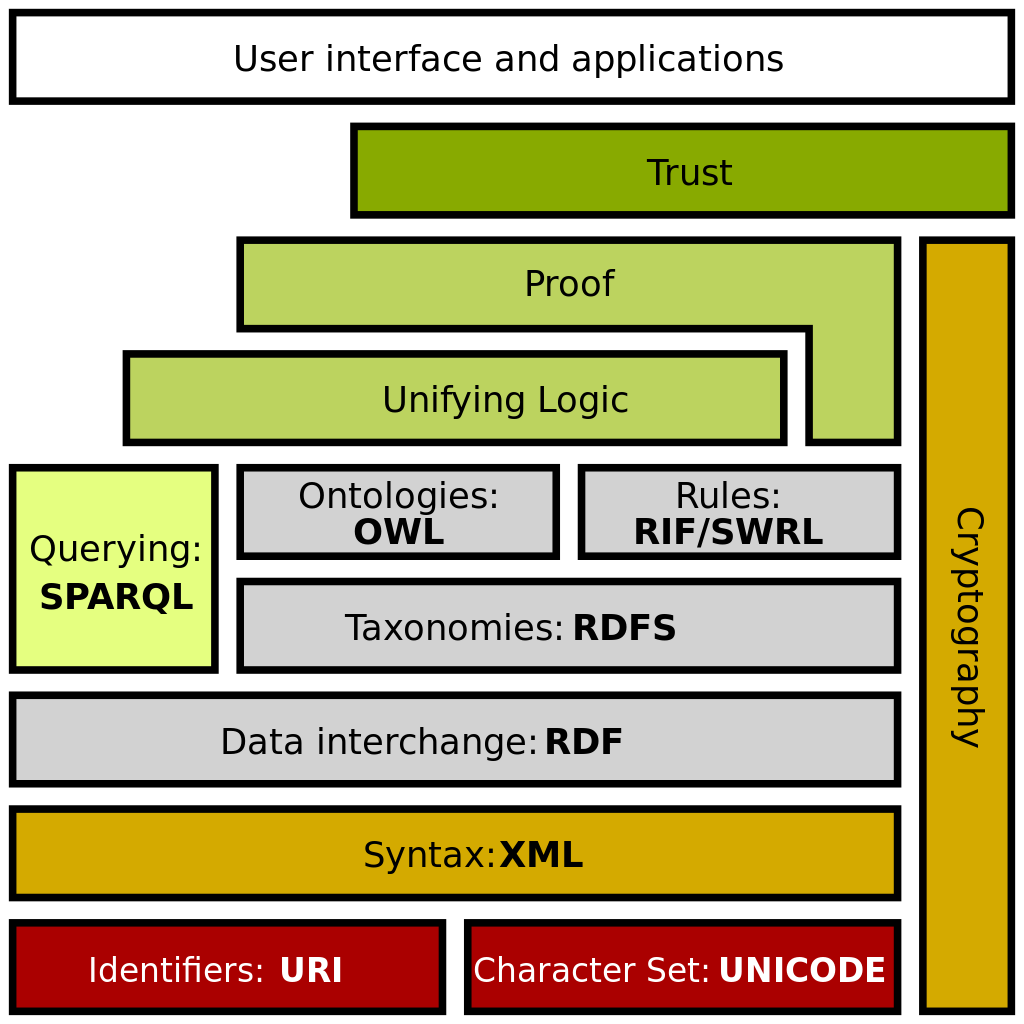
\includegraphics[width=0.65\textwidth]{img/web_stack.png}  
    \caption[Visualisierung eines Graphen auf Basis eines RDF-Datensatz, \protect\url{https://www.w3.org/TR/rdf11-primer/}, 10.04.2019.]{Visualisierung eines Graphen auf Basis eines RDF-Datensatz.}
  	\label{fig:web_stack}
\end{figure}

Das Semantic Web ist nicht erreicht. Zumindest nicht für die Allgemeinheit. Die großen Internetriesen hingegen verfügen über ''ihre Semantic Web'', in denen sie ihre eigenen Agenten mit ihrer großen Datenmenge arbeiten lassen.\footnote{\url{https://twobithistory.org/2018/05/27/semantic-web.html}}




%%%%%%%%%%%%%%%%%%%%%%%%%%%%%%%%%%%%%%%%%%%%%
%%%%%%%%%%%%%%%%%%%%%%%%%%%%%%%%%%%%%%%%%%%%%
\subsubsection{Resource Description Framework}

Das \textit{Resource Description Framework} (RDF) ist ein Datenmodell zur Darstellung und für den Austausch von Daten im Web. Daten werden in diesem Modell als Ressourcen definiert, wobei eine Ressource alles sein kann: ein Dokument, eine Person, ein physisches Objekt oder ein abstraktes Konzept. Über Ressourcen werden Statements der Form Subjekt-Prädikat-Objekt formuliert. Jedes Statement drückt eine Beziehung zwischen zwei Ressourcen aus. Das Subjekt und das Objekt stehen dabei für die beiden miteinander verbundenen Ressourcen; das Prädikat beschriebt die Art ihrer Beziehung. Diese Zusammensetzung von Subjekt, Prädikat und Objekt werden als Triples bezeichnet. Betrachtet man den Satz ''\textit{Bob ist befreundet mit Alice}'', dann lässt sich folgendes Triple extrahieren: \textit{<Bob>} als Subjekt, \textit{<ist befreundet mit>} als Prädikat und \textit{<Alice>} als Objekt. Ob \textit{Alice} mit \textit{Bob} befreundet ist geht aus diesem Statement noch nicht hervor, da jeder Relation in RDF nur eine Richtung definiert.\footcite[Vgl.][S.16-21]{powers2003practical} In der graphischen Darstellung wird schnell klar, dass es sich beim RDF Datenmodell um einen gerichtete Graphen handelt, der aus Knoten (Subjekt und Objekt), sowie aus Kanten (Prädikat) besteht, wie Abbildung \ref{fig:triple} zeigt.
\begin{figure}[h]
  \centering
	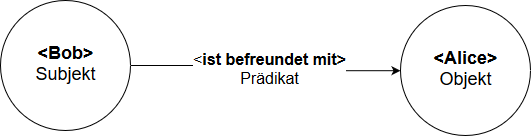
\includegraphics[width=0.75\textwidth]{img/triple.png}  
    \caption[ Semantic Web Stac]{ Semantic Web Stac}
  	\label{fig:triple}
\end{figure}
SCHREIBER und RAIMOND\footcite[Vgl.][]{schreiber2014rdf} erklären RDF in einem ausführlichen Beispiel an Hand folgenden Aussagen:
\\
\\
\textit{Bob ist eine Person.\\
Bob ist befreundet mit Alice.\\
Bob ist geboren am 4. Juli 1990. \\
Bob interessiert sich für die Mona Lisa.\\
Die Mona Lisa wurde von Leonardo da Vinci entworfen.}
\\
\\
Jede dieser Zeilen steht für ein Triple. \textit{Bob} ist Subjekt in vier der oben genannten Tripeln, \textit{Mona Lisa} tritt zweimal als Objekt und einmal als Subjekt auf. Dies ermöglicht es eine beliebige Menge an Triple zu einem komplexeren Graphen zusammenzusetzen und somit komplexere Sachverhalte beschreiben zu können. Abbildung \ref{fig:rdf_example} veranschaulicht das.
\begin{figure}[h]
  \centering
	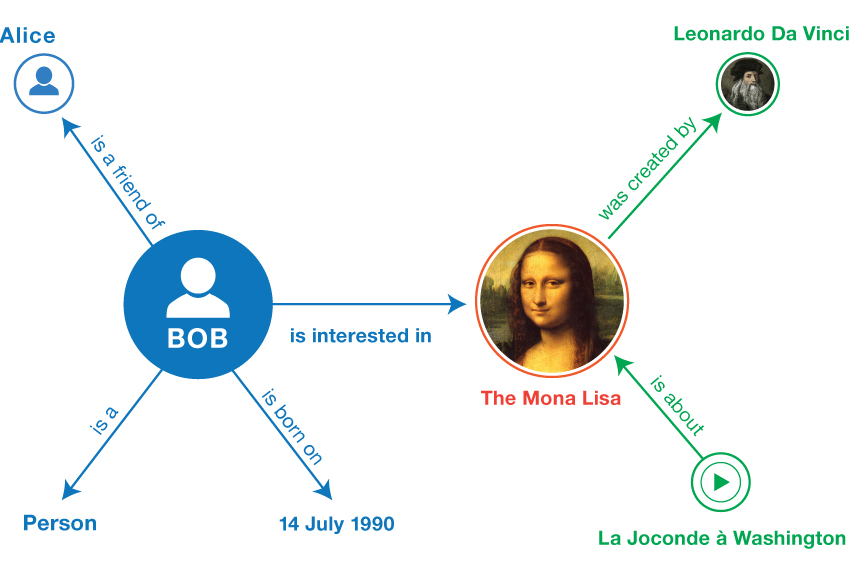
\includegraphics[width=1\textwidth]{img/rdf_example.png}  
    \caption[Visualisierung eines Graphen auf Basis eines RDF-Datensatz, \protect\url{https://www.w3.org/TR/rdf11-primer/}, 10.04.2019.]{Visualisierung eines Graphen auf Basis eines RDF-Datensatz.}
  	\label{fig:rdf_example}
\end{figure}
\textbf{\textit{Uniform Resource Identifier}(URI)} können in allen drei Positionen eines Triple erscheinen. Somit ist jeder Ressource, sowie jeder Beziehung zwischen Ressourcen durch eine URI identifizierbar. URI's sind durch ein erweiterbares Schema definiert, damit Ressourcen im Internet eindeutig adressiert werden können. Um dabei die Einheitlichkeit zu gewährleisten, folgen sie einem vordefinierten Satz von Syntaxregeln, der 5 Komponenten beinhaltet:\footcite[Vgl.][]{berners2004uniform}
\begin{center}
\textit{URI = scheme:[//authority]path[?query][\#fragment]}
\\
\end{center}
\begin{itemize}
\item \textbf{\textit{scheme}}: Definiert den Kontext und Typ. Bekannte Schemata sind beispielsweise die Webprotokolle \textit{Hyper Text Transfer Protocol} (http) oder das \textit{File Transfer Protocol} (ftp), sowie Notationskonzepte wie \textit{Uniform Resource Name} (URN)urn oder \textit{Digital Object Identifier} (doi).
\item \textbf{\textit{authority}}: Verwaltet Instanz in einem bestimmten vom Schema angegebenen Interpretationsraum, wie etwa das \textit{Domain Name System}.
\item \textbf{\textit{path}}: Der Pfad enthält – oft hierarchisch organisierte – Angaben, die zusammen mit dem Abfrageteil eine Ressource identifizieren. 
\item \textbf{\textit{query}}: Der Abfrageteil beinhaltet Daten zur Identifizierung von solchen Ressourcen, deren Ort durch die Pfadangabe allein nicht genau angegeben werden kann, wie beispielsweise ein Datensatz aus einer Datenbank, abgerufen werden
\item \textbf{\textit{fragment}}: Ist der optionale Fragmentbezeichner und referenziert eine Stelle innerhalb einer Ressource. Der Fragmentbezeichner bezieht sich immer nur auf den unmittelbar vorangehenden Teil des URI und wird von einem Hash (\#) eingeleitet.
\end{itemize}

Weiters werden URI in \textit{Uniform Resource Locator} (URL) und \textit{Uniform Resource Name} (URN) unterteilt. Wo URN Namen von Ressourcen eindeutig indetifuieren, wie etwa bei ISBN Nummern von Büchern, sind URL die gägnisten URI's, die den Ort einer Ressource addressieren und über einen Webbrowser auch aufrufen können.\footcite[Vgl.][S.21-22]{powers2003practical} Für das Triple \textit{<Bob>} \textit{<interessiert sich für>} \textit{<die Mona Lisa>} wird jeder Teilbestand eine URI und in der \textit{Turtle} Serialistion von RDF ergibt es folgenden Code:
\begin{lstlisting}[]
BASE   <http://example.org/>
PREFIX foaf: <http://xmlns.com/foaf/0.1/>
PREFIX xsd: <http://www.w3.org/2001/XMLSchema#>
PREFIX schema: <http://schema.org/>
PREFIX dcterms: <http://purl.org/dc/terms/>
PREFIX wd: <http://www.wikidata.org/entity/>

bob#me a foaf:Person ;
         foaf:knows <alice#me> ;
         schema:birthDate "1990-07-04"^^xsd:date ;
         foaf:topic_interest wd:Q12418 .
 
wd:Q12418 dcterms:title "Mona Lisa" ;
            dcterms:creator <http://dbpedia.org/resource/Leonardo_da_Vinci> .
\end{lstlisting}

%%%%%%%%%%%%%%%%%%%%%%%%%%%%%%%%%%%%%%%%%%%%%
%%%%%%%%%%%%%%%%%%%%%%%%%%%%%%%%%%%%%%%%%%%%%
\subsubsection{Resource Description Framework Schema (RDFs)}

Im vorhergehenden Beispiel wurden \textit{<Bob>} und \textit{<Alice>} der Klasse \textit{<Person>} zu geordnet. Sie sind Instanzen der Klasse \textit{<foaf:Person>}. Desweiteren wurde eine Relation zwischen diesen beiden Personen definiert: \textit{Bob ist befreundet mit Alice}.
\\
Um die Beziehungen zwischen Ressourcen zu beschreiben liefert das \textbf{Resource Description Framework Schema (RDFs)} eine semantische Erweiterung für RDF. Dies umfasst die Möglichkeit Klassen und Relationen, so genannte Properties, zu definieren und folgt dem Paradigma der Objektorientierung. Es lassen sich auf dieswe Weise Instanzen von Klassen erzeugen, die alle Eigenschaften der Klasse und ihrer übergeordneten Klassen erben. Blickt man auf das FOAF-Vokabular\footnote{FOAF-Specification, \protect\url{http://xmlns.com/foaf/spec/ }, 29.05.2019.}, das als RDFs umgesetzt ist, so kann man feststellen, dass \textit{foaf:Person} eine Unterklasse von \textit{foaf:Agent} ist. Weitere Unterklassen davon sind \textit{foaf:Group} und \textit{foaf:Organization}. Alle drei Unterklassen haben bestimmte Eigenschaft gemeinsam: sie setzen Handlungen in der Welt. Sie unterscheiden sich aber in den Relationen mit denen sie selbst, oder in Abgrenzung zu anderen Klassen, beschrieben werden können. Eine \textit{foaf:Group} besteht aus mehrern \textit{foaf:Person}. Dies wird mittels der Property \textit{foaf:member} ausgedrückt. Im Gegenzug verfügt \textit{foaf:Person} über eine Relation \textit{foaf:knows}, die ausdrückt, dass sich zwei Personen kennen. Die Richtung dieser Relation - wer wen kennt - wird mit den in RDFs mittels den Termen \textit{rdfs:Domain} und \textit{rdfs:Range} definiert. 
Für \textit{foaf:knows} wird \textit{Domain} und \textit{Range} auf die Klasse\textit{ foaf:Person} gesetzt: eine Person kennt eine andere Person. Für die Property \textit{foaf:member} wird \textit{Domain} auf \textit{foaf:Group} und \textit{Range} auf \textit{foaf:Person} gesetzt: eine Gruppe besteht aus Personen.
\\
Weiter führt RDFs Datentypen ein. Damit lässt sich beschreiben, um welche Art eines Literals es sich handelt. Es kann für die maschinelle Verarbeitung sehr wichtig sein zu wissen, ob es sich um eine Zeichenkette, eine Zahl, eine Datumsangabe oder eine XML Struktur handelt, da mit unterschiedlichen Datentypen andere Operationen einhergehen. 
\\
Mit den RDF Properties \textit{rdfs:label} und \textit{rdfs:comment} lassen sich Properties und Classes benennen und beschreiben. Das ist deswegen nötig, da der Fokus einer Klasse nur in bestimmten Kontexten Sinn macht. \textit{rdfs:label} definiert einen menschenlesbaren Namen einer Ressource. Es besteht stets die Möglichkeit in RDF die einzelnen Lables einer Ressource mit Sprachkürzel zu versehen. Die Property \textit{rdfs:comment} erlaubt es eine verbale Beschreibung zu einer Klasse hinzuzufügen.Am Beispiel von \textit{foaf:Person} ist das das Label ''Person'' und die Beschreibung:\\
'\textit{The Person class represents people. Something is a Person if it is a person. We don't nitpic about whether they're alive, dead, real, or imaginary. The Person class is a sub-class of the Agent class, since all people are considered 'agents' in FOAF. }''.\\
Daneben existiert auch ein Konstrukut \textit{rdfs:seeAlso}, um ausdrücken, dass es unter folgender URL noch weitere Information zu dieser Ressource gibt.\footcite{brickley2014rdf} Folgender Darstellung veranschaulicht die soeben beschriebenen Konstrukte in RDFs und zeigt Unterklassen der Superklasse \textit{foaf:Agent}, zwei Instanzen der Klasse \textit{foaf:Person} und stellt graphisch - durch den Pfeil - \textit{Domain} und \textit{Range} einer Propertie dar. 
\begin{figure}[H]
  \centering
	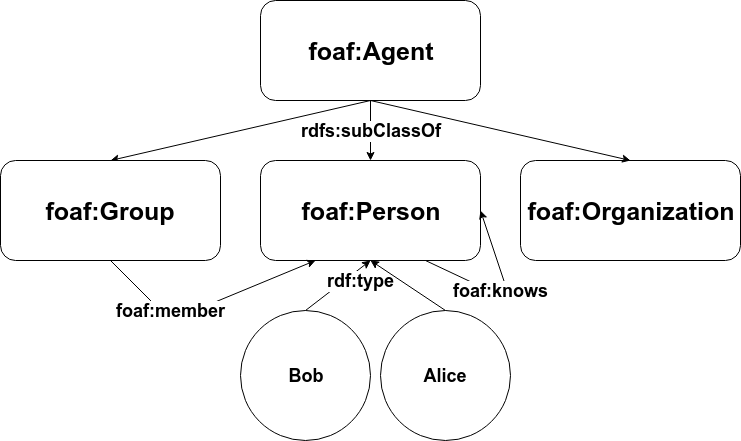
\includegraphics[width=0.75\textwidth]{img/rdfs.png}  
    \caption[RDFs-Beispiel auf Basis des FOAF-Vokabulars, eigene Darstellung.]{RDFs-Beispiel auf Basis des FOAF-Vokabulars}
  	\label{fig:web_stack}
\end{figure}
Hinter jeder Klasse, Property und  jeder Instanz steht eine URI. Folgendes RDF-Snippet zeigt wie die Klasse \textit{foaf:Person} und \textit{foaf:knows} im FOAF-Vokabular mittels RDFs definiert werden.
\begin{lstlisting}[]
@prefix rdfs: <http://www.w3.org/2000/01/rdf-schema#> .
PREFIX foaf: <http://xmlns.com/foaf/0.1/>
@prefix rdf: <http://www.w3.org/1999/02/22-rdf-syntax-ns#> .

foaf:Person a rdfs:Class ;
  rdfs:label "Person" ;
  rdfs:comment "A person." ;
  rdfs:subClassOf foaf:Agent .
  
foaf:knows a rdf:Property;
  rdfs:label "knows" ;
  rdfs:comment "A person known by this person (indicating some 
  level of reciprocated interaction between the parties)." ;
  rdfs:domain foaf:Person ;
  rdfs:range foaf:Person .
\end{lstlisting}

ToDo Hitzler\footcite[][]{hitzler2007semantic} 

%%%%%%%%%%%%%%%%%%%%%%%%%%%%%%%%%%%%%%%%%%%%%
%%%%%%%%%%%%%%%%%%%%%%%%%%%%%%%%%%%%%%%%%%%%%
\subsubsection{Taxonomien: Simple Knowledge Organisation (SKOS)}


%%%%%%%%%%%%%%%%%%%%%%%%%%%%%%%%%%%%%%%%%%%%%
%%%%%%%%%%%%%%%%%%%%%%%%%%%%%%%%%%%%%%%%%%%%%
\subsubsection{Abfragesprache: SPARQL}
Wie man in der Welt der relationalen Datenbanken mit der Abfragesprache SQL Datenbankabfragen formulieren kann, so kann man mit \textit{SPARQL Protocol And RDF Query Language} RDF Daten bzw. Triple in Graphdatenbanken abfragen.\footcite[][]{w3c2013sparql}
\\
Folgendes Snippet einer SPARQL-Abfrage zeigt die Syntax dieser Abfragesprache. Ziel dieser Abfrage ist es, alle Ressourcen in einer Graphdendatenbank abzufragen, die über eine \textit{foaf:name} und eine \textit{foaf:knows} Propertie verfügen. Das Ergebnis wird nach den Personen und Namen gruppiert, also es werden keine Dupletten von URI's zurückgegeben. Als Ausgabe erfolgt eine Tabelle (bzw. eine XML, JSON oder CSV Datenformat) in der die Namen und die Anzahl der Freunde, definiert als alle Knoten auf die \textit{foaf:know} referenziert.
\begin{lstlisting}[]
PREFIX foaf: <http://xmlns.com/foaf/0.1/>
SELECT ?name (COUNT(?friend) AS ?count)
WHERE { 
    ?person foaf:name ?name . 
    ?person foaf:knows ?friend . 
} GROUP BY ?person ?name
\end{lstlisting}
Mit PREFIX werden die Namespaces definiert. Das reservierte Wort \textit{SELECT} definiert alle Variabeln, diese werden durch ein vorangestelltes Fragezeichen gekennzeichnet, die als Rückgabewert definiert werden. Daneben gibt es in der SPARQL1.1 Version Operatoren und Funktionen, wie etwas \textit{COUNT()}, das alle Treffer der \textit{?friend} Variabel zählt und in der \textit{?count Variabel} speichert. Im \textit{WHERE} Bereich werden alle Bediengungen für die Abfrage definiert. Diese Bedienungen entsprechen der Definition eines Teilgraphen, der wiederum eine Teilmenge des gesamten Datenbestandes abbildet. Hier stehen weiter Konstrukte wie \textit{OPTIONAL}, einem logischen Oder, so wie \textit{UNION} einem logischen Und zur Verfügung. Über eine SPARQL-Endpoint können so User über das Web Datenbestände abfragen und mit diesen Arbeiten.\footcite[][S.1-45]{ducharme2013learning}  Ein bekanntes Beispiel dafür ist der Endpoint von Wikidata.

%%%%%%%%%%%%%%%%%%%%%%%%%%%%%%%%%%%%%%%%%%%%%
%%%%%%%%%%%%%%%%%%%%%%%%%%%%%%%%%%%%%%%%%%%%%
\subsection{Ontologien}
ToDO
\\
formationsmodelle umfassen die Verwendung einer expliziten Sprache zur Informationsdarstellung.\footcite{kobler2010qualitat} 
\\
\\
Der Gegenstandsbereich der \textbf{Ontologie als Disziplin in der Philosophie} umfasst alles, das existiert. Das Erkenntnisziel, so MEIXNER, ist auf allgemeiner begrifflicher Ebene zu finden und beschäftigt sich mit der Einteilung des Seins und den Grundstrukturen der Wirklichkeit, sowie der Frage nach dem Wesen der Existenz. Die Ontologie verfolgt nicht das Ziel Erkenntnis über ein Objekt zu erhalten, es beispielsweise zu vermessen oder zu beschreiben, sondern stellt sich die Frage nach welchen allgemeinen Kriterien Objekte im Verhältnis zu ontologischen Begriffen wie Sein, Aktualität, Universalie, Exemplifikation, Sachverhalt oder Individuum stehen.\footcite{meixner1994wissenschaft}
\\
Der Begriff \textbf{Ontologie in der Informationswissenschaft bzw. Informatik} umfasst ein pragmatisches Konzept zum Austausch und zur Wiederverwendung von formalisierten und gemeinschaftlich verwendeten Wissensstrukturen durch ein gemeinsames Vokabular. Ziel dabei ist es Informationssysteme zu implementieren. Die Spezifikation eines solchen Vokabulars für eine bestimmte Domäne nennt man Ontologie.
\\
Der Begriff wird in zwei Disziplinen mit jeweils unterschiedlichen Fokus verwendet. Dennoch sehe ich Gemeinsamkeiten. Beide setzen sich mit der Frage auseinander, wie  die Welt sinnvoll strukturiert werden kann, damit wir uns besser darin zurecht finden können. In diesem Kapitel wird die informationswissenschaftlichen Dimension des Ontologie-Begriffs und seiner Nutzung in den digitalen Geisteswissenschaften diskutiert und der Frage nachgehen, ob Ontologien ein geeignetes Werkzeug zur Formalisierung von geschichtswissenschaftlichen Domänen darstellen. Dabei soll anfangs "Wissen" kurz aus informationswissenschaftlicher Sicht definiert werden und über das semantische Netz eine Brücke zur Ontologie geschlagen werden. 

%%%%%%%%%%%%%%%%%%%%%%%%%%%%%%%%%%%%%%%%%%%%%
%%%%%%%%%%%%%%%%%%%%%%%%%%%%%%%%%%%%%%%%%%%%%
\subsubsection{Vom Wissen, über das Semantische Netz zur Ontologie}
\textbf{Wissen} ist eine systeminterne Repräsentation vorliegender Erfahrungen eines Menschen zu einem bestimmten Zeitpunkt, die einem zu überprüfenden Anspruch auf Gültigkeit ausgesetzt sein muss. Als solches prägt Wissen das Handeln und Denken eines Menschen auf den unterschiedlichsten Ebenen und dient zur Lösung von Problemen. Das jeweils aktuelle Wissen bildet einen kontextuellen Rahmen, in dem ankommende und bestehende Information interpretiert und zu neuen Erfahrungen verarbeitet werden.\footcite{favre2001information}
\\
Diese Definition von Wissen -- eine stärker informationswissenschaftliche -- hat seinen, neben vielen Definitionen in anderen Fachbereichen, legitimen Ursprung.  Unterschiedlichen Disziplinen haben andere Fragestellungen und benötigen dafür ein anderes theoretisches Gerüst. Ein Wissensbegriff in der Philosophie, beispielsweise, sollte viel weiter gefasst sein, als ein Wissensbegriff in der Informationswissenschaft, dessen Aufgabe darin besteht als Hilfsmittel in der Entwicklung und Umsetzung von Informationssystemen zu fungieren. 
\\
\\
Mittels Ontologie lässt sich ''Wissen'' als Netzwerk beschreiben. Ein Netzwerk ist ein gerichteter Graph, bestehend aus einer Menge von Knoten und einer Menge von Kanten, die die einzelnen Knoten miteinander verknüpfen. Damit lassen sich (fast) beliebige Entitäten und deren Verknüpfungen miteinander abbilden. Die Überlegungen zu einem \textbf{semantischen Netz}, als gedanklichen Vorgänger der Ontologie, stammen von QUILIIAN, der damit ein formales Erklärungsmodell für '\textit{die menschliche Repräsentation von Wissen über Worte und ihre Bedeutung als Netzwerk von Begriffen und ihren Relationen}' \footcite{stuckenschmidt2009ontologien} beschreibt. Semantische Netze können einen Kompromiss zwischen menschenverständlicher Repräsentation einer Domäne  und der formalen Verarbeitbarkeit durch eine Maschine darstellen.\footcite{reichenberger2010grundlagen} Das ist dadurch gegeben, dass die Struktur des Graphen (=Netz), sich einfach in Rechnern als Matrizen abbilden lässt.
\\
Die Ontologie ist eine Erweiterung des semantischen Netzes und nach GRUBER kann sie durch ein \textbf{4-Tupel} definiert werden. C ist eine Menge von \textbf{Klassen} (concepts, classes - Mengen von Entitäten aus der Realität), R eine Menge von \textbf{Relationen} (properties - Beziehungen zwischen Klassen), I eine Menge von \textbf{Instanzen} (individuals - einzelne Entität aus einer Menge) und A eine Menge von \textbf{Axiomen} (axioms - logische Regel).\footcite{joostbreukera2009flood} C und R lassen sich dabei stets als Graph abbilden. Ein Beispiel zur Veranschaulichung: 
\\
Es existiert eine Klasse (C) "Katzen", die mit der Relation "ist ein" (R) mit einer Klasse "Säugetier" verbunden ist.  Die Individuals (I) "Garfield“ und "Tom" sind Instanzen der Klasse "Katzen" und erben alle Eigenschaften, die in der Klasse "Katzen" definiert wurden. Eine Regel kann definiert werden (A), sodass immer wenn eine Klasse eine "ist ein" Verbindung zu einer Klasse wie "Säugetier" hat, es ausgeschlossen ist, dass es eine zweite "ist ein"-Verbindung  gibt, die auf eine andere Klasse wie etwa "Vögel" referenziert. 
\\
\\
Der Begriff der Ontologie terminologisch unscharfe verwendet.\footcite[Vgl.][S.1]{gruber1993translation} Die Unterschiede sind klein, aber dennoch entscheidend und sollen im Folgenden diskutiert werden.
Eine der  ersten  Definitionen des Begriffs der Ontologie stammt von GRUBER: 
\begin{center}
 "\textit{An ontology is    an    explicit    specification    of    a conceptualization}
"\footcite[][S.69]{hoekstra2009ontology}
\end{center}
Eine "\textit{conceptualization}" beschreibt den Prozess einer Vereinfachung, aber Fokussierung, eines bestimmten Aspekts der Realität. 
So kann eine Ontologie als Dokumentation eines 
wissen- schaftlichen 
Prozesses agieren, in dem die Wirklichkeit abstrahiert und reduziert wird und gleichzeitig die Domäne bzw. Forschungsfrage hervorgehoben und amplifiziert wird.\footcite[Vgl.][]{thaller2017ungefahre}
Unter "\textit{explicit}" versteht man, dass die Bedeutungen aller von der Ontologie erfassten Begriffe klar und eindeutig definiert sein müssen. Dies beinhaltet alle ihre Eigenschaften, Beschränkungen und Beziehungen, innerhalb, als auch außerhalb der Domäne.\footcite{sure2003methodology}
BORST erweitert GRUBERS Definition um  '\textit{formal  specification  of  a shared  conceptualization}'.\footcite{borst1997construction}
"\textit{Formal}" ergänzt dabei die Definition um die Notwendigkeit, dass Ontologien maschinenlesbar sein müssen. Erst diese Eigenschaft hebt sie von anderen Methoden zur Formalisierung von konzeptionellen Datenmodellen hervor. Der Zusatz "\textit{shared}" reflektiert die Tatsache, dass eine Ontologie Wissen erfasst, das durch den Konsens einer Gruppe - z.B. durch einen wissenschaftlichen  Diskurs - akzeptiert wird. Eine Ontologie darf nicht im Stillen von einer Person alleine entwickelt werden, sondern sollte in einem iterativen Prozess (Ontology Engineering) des Austausches und der Diskussion mit anderen entstehen. Ein solcher Prozess kann wie folgt ablaufen:
\begin{itemize}
\item Definition der Notwendigkeit und des Zieles einer Ontologie
\item Strukturierung des Wissens und konzeptionelle Entwicklung
\item Implementierung und Modellierung
\item Evaluierung und Dokumentation
\item Iteration dieser Punkte im Austausch mit anderen
\end{itemize}
Allgemeiner betrachtet definieren LINCKELS \& MEINEL eine Ontologie als ein Datenmodell zur Darstellung eines Sets miteinander vernetzter Konzepte innerhalb einer (Fach-)Domäne.\footcite{linckels2011librarian}
WELLER spricht von einer formalen und schematischen Darstellung einer Wissensdomäne auf Basis definierter Regeln und Vokabulars.\footcite{weller2013InformationBand}
\\ 
Zusammengefasst kann man sagen, dass sich mittels Ontologien komplexere Sachverhalte so darstellen lassen, dass Mensch und Maschinen in der Lage sind Strukturen, die durch eine Ontologie definierte und standardisierte sind, weiterverarbeiten zu können. Der Mehrwert kann vor allem in der Möglichkeit automatisierter Schlussfolgerungen, im Information Retrieval oder anderen formalen Methoden zur Verarbeitung von Daten liegen.
\\
\\
Der Ontology Editor Protégé erlaubt es, eine Ontologie und die darin enthaltenen Daten (Individuals) einem Reasoning - dem Abarbeiten aller Vorhanden Regeln in einer Ontologie auf Basis einer deskriptiven Logik - zu unterziehen. Für solche Zwecke gibt es natürlich auch API's und Bibliotheken in Programmiersprachen.\footcite{musen2015protege} Das Reasoning gilt als ein essentieller Baustein im Design, der Entwicklung, der Wartung und in der praktischen Anwendung einer Ontologie. Das Ergebnis davon sind Inferenzen. Inferenzen sind neu hergeleitete Schlussfolgerungen auf Basis der formalen Regeln einer Ontologie.\footcite{dentler2011comparison} Die Überprüfung strukturierter Daten mittels logischen Schlussfolgerungen kann dazu dienen, größere Datenmengen auf ihre Konsistenz und somit auch auf ihre Qualität hin zu prüfen, da logische Inkonsistenzen als Fehlermeldung angezeigt werden.
\\
\\
huhu Ontologie zitieren\footcite[Vgl][S.162-178]{jannidis2017digital} 

\subsubsection{Ontology Engineering}

\subsubsection{Reasoning}

\subsubsection{Linked Open Data}

\section{Historische Rechnungsbücher als Quelle}

Historische Rechnungsbüchern sind einen Teil einer Menge von Primärquellen, die Aufzeichnungen von Handel mit Waren und Dienstleistungen darstellen. Sie werden seit längerer Zeit als Primärdatensätze für historische Forschung genutzt. Sie liefern reichhaltige und strukturierte Daten, die oft längere Zeiträume abdecken und die als Aggregation vieler Einzelinformationen enthalten zu Beantwortung unterschiedlicher Forschungsfragen herangezogen werden können. Sie beinhalten beispielsweise Information über den Kauf und Verkauf von Waren, Werkzeugen und Rohstoffen eines bestimmten Gewerbes, sowie über die ausgezahlten Löhne von Arbeitnehmern*innen. Eine andere Art von Rechnungsbüchern stellen Haushaltskonten dar. Diese beziehen sich auf den Kauf von Lebensmittel und Bekleidung sowie für Zahlungen für Dienstleistungen in Form von Kochen, Waschen oder andere Haushaltsarbeiten.   HFRs im Zusammenhang mit der Haushaltsführung auch im Zusammenhang mit der Haushaltsführung enthalten Listen der für Hausarbeit gezahlten Löhne, und solche Listen finden sich manchmal auf der Seite Rückseiten von Taschenkalendern und nicht in formalen Kontenbüchern oder Ledgern. In Regionen wo Arbeiter versklavt wurden, finden sich HFRs in den Buchhaltungsbüchern und in der persönlichen Aufzeichnungen über Sklavenhalter und Sklavenhändler.\footcite[][S.2]{tomasek2013encoding}
\\
Eine Transkription allein reicht nicht aus um die unterschiedlichen Dimensionen einer solchen Quelle abzudecken: die linguistische/textuelle, die quantifizierbare und die semantische Dimension. Für Forschungszwecke unterliegen historische Quellen einem Transformationsprozess hin zu (vernetzten) Informationsquellen, die in verschiedenen Forschungsszenarien genutzt werden können. Um dies zu veranschaulichen, werden drei Fallstudien von Projektpartnern und ihren jeweiligen Forschungsinteressen diskutiert, die weit über wirtschaftliche und administrative Aspekte hinausgehen.
\\
\\
Händler haben finanzielle Aufzeichnungen geführt, um Käufe und Verkäufe von Waren seit den Handelsökonomien des alten Mesopotamiens zu verfolgen, und der Impuls, regelmäßige Konten zu führen, führte zu Standards für die Erfassung von Finanzinformationen. Im Laufe der Jahrhunderte boten verschiedene einflussreiche Texte gewöhnlichen Geschäftsleuten die Möglichkeit, zu lernen, wie man das macht. Für das frühneuzeitliche Europa skizzierte Fra Luca Pacioli in seiner Abhandlung The Rules of Double-Entry Bookkeeping von 1494 Rechnungslegungsgrundsätze, die die Handelsrechnung in ganz Europa beeinflussten. Mitte des achtzehnten Jahrhunderts veröffentlichte der schottische Mathematiker John Mair ein einflussreiches Lehrbuch mit dem Titel 
Buchhaltungsmethodik; oder, eine methodische Abhandlung von Handelskompten, nach der italienischen Form. Bei der Präsentation von Pacioli's System für Englischsprachige durchlief Mair's Text zahlreiche Ausgaben zwischen den folgenden Sprachen 1736 und 1808. \footcite[][S.3]{tomasek2013encoding}

%%%%%%%%%%%%%%%%%%%%%%%%%%%%%%%%%%%%%%%%%%%%%
%%%%%%%%%%%%%%%%%%%%%%%%%%%%%%%%%%%%%%%%%%%%%
\subsection{DEPCHA}

Daten - aus unterschiedlichen Formaten - sollen auf einer gemeinsamen Plattform zusammengeführt werden und adäquate Formen des Retrievals, Discoverys und der Visualisierung eröffnen, um die Arbeit mit den Quellen zu erleichtern. Die Überführung nach RDF auf Basis der im Projektkontext entwickelten \textit{Bookkeeping-Ontologie}, die Transferprozesse historischer Rechnungsbücher formalisiert, erlaubt die Interoperabilität, Verlinkung und Zusammenführung der Informationen im Sinne des \textit{Web of Data} und \textit{Linked Open Data}.


\subsection{The George Washington Financial Papers}
The George Washington Financial Papers (1748-1799) 3 gives insight into the life of
George Washington and other topics such as the material culture, social history,
manufacturing and agriculture. The financial papers exist as digital edition, created and
published via an open-source, Drupal 4 based editorial platform, and aim to make
Washington’s records freely accessible. The platform allows editing and publishing
financial documents and gives the users the possibility to perform simple analytical
functionalities. Samples of research questions that could be of interest to historians are:
How much money did Washington spent annually and for which specific commodities?
Which role slave trade plays in his business? How did the price of certain commodities
fluctuate? What did the network of partners look like and who did business with him?
How was the value of tobacco calculated through different currencies [St14]?

\subsection{The Wheaton Accounts}

Die \textit{Wheaton Family Papers} umfassen mehrere Bücher im Zeitraum von 1828 bis 1859, die unter anderem die finanziellen Geschäfte von \textit{Laban Morey Wheaton} und seiner Familie, einem Geschäftsbesitzer eines \textit{dry goods store} aus Norton, Massachusetts in den Vereinigten Staaten von Amerika, dokumentieren. Unter \textit{dry goods} versteht man einen aus dem 17. Jahrhundert stammenden historischen Begriff, der je nach Region leicht unterschiedliche Güter zusammenfasst. Darunter werden im Allgemeinen aber Produkte verstanden, die ''trocken'' sind, wie etwa Textilien, Konfektionskleidung, Tabak oder bestimmten Lebensmittel, wie etwa Kartoffel.\footcite[Definition von \textit{Dry Goods}, \protect\url{https://chestofbooks.com/reference/Dictionary-of-Dry-Goods/Dry-Goods.html}, 23.05.2019, Vgl.][]{cole2015complete}
\\
Die Stadt Norton ist eine charakteristische landwirtschaftlich und von Manufakturen geprägte Kleinstadt im Nordosten der USA im Hinterland der regional bedeutenden Häfen Boston, New Bedford, Newport, and Providence. In einer Geschichte der Stadt Norton von CLARK wird \textit{Laban Morey Wheaton} namentlich genannt. Er lebte von 14.September 1796 bis 1865, hat Rechtswissenschaften an der \textit{Brown University} studiert und jahrelang als \textit{Postmaster of Norton} gearbeitet. Er war politisch aktiv und war Vertreter im \textit{Massachusetts General Court}, sowie Mitglied im \textit{Massachusetts Governor's Council}. Er war verheiratet und Angehöriger des Kongregationalismus, einer Form der christlichen Gemeindeverfassung. Die Wheaton Familie besaß eine Milchviehherde sowie eine Fabrik zur Produktion von Baumwollwatte und Strohhüten\footcite[][S.6]{tomasek2013encoding} und so gehörte Laban Wheaton zu einem der wohlhabendes Männer der Stadt. Sogar ein Portrait von ihm ist bei CLARK überliefert.\footcite[][S.496]{clark1859history} 
\begin{figure}[H]
\centering
	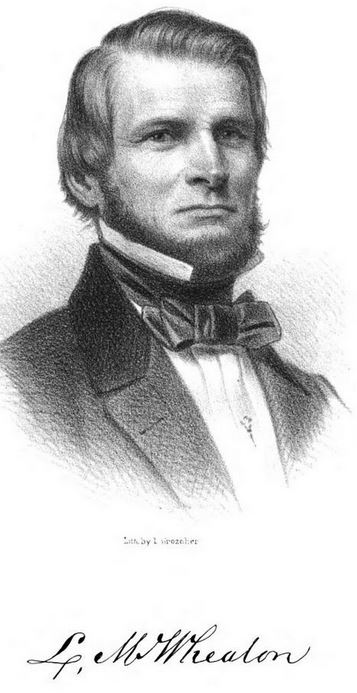
\includegraphics[width=0.2\textwidth]{img/LMwheaton.jpg}  
    \caption[Portrait von Laban Morey Wheaton, Vgl. CLARK, George Faber: A History of the Town of Norton, Bristol County, Massachusetts, from 1669-1859.
Crosby, Nichols, and Company, and author at Norton, 1859, S.497.]{Portrait von Laban Morey Wheaton} \label{fig:LMwheaton}
\end{figure} 
Aus diesem Kontext heraus, der über \textit{Laban Morey Wheaton} überliefert ist kann man die These aufstellen, dass er ein mächtiger Mann war. Auf der einen Seite politisch aktiv und politischer Vertreter, auf der anderen Seite vermögend und Besitzer mehrere Immobilien und eines Geschäftes. Gerade der im \textit{daybook} dokumentierte Verkauf von Gütern, in dem Menschen Lebensmittel im Austausch für Arbeit erwerben, zeigt eine gewisse Machtposition.
\\
\\
Das \textit{Wheaton College Massachusetts} stellt die \textit{Wheaton Family Papers} Dokumente in ihrem digitalen Repositorium online zur Verfügung.\footnote{Wheaton Family Papers, \url{https://digitalrepository.wheatoncollege.edu/handle/11040/7928}, 19.05.2019.} 
\\
Die wissenschaftliche Auseinandersetzung erfolgt durch Kathryn Tomasek, Professorin für Geschichte am \textit{Wheaton College Massachusetts}. Im Zuge des Projektes \textit{The Wheaton College Digital History Project} wurden Teile der Wheaton Paper, darunter beispielsweise das oben angeführte \textit{daybook} gemeinsam mit Studierenden transkribiert und mit dem Standard der Text Encoding Iniative (TEI) ausgezeichnet und im Sinne einer Vorarbeit einer digitalen Edition ediert. Der Fokus dieser Arbeiten liegt auf der Erschließung der einzelnen Transaktionen und der damit verbundenen Personen, Güter und Dienstleistungen.\footcite[Vgl. TOMASEK Kathryn: The Wheaton College Digital History Project: Undergraduate Research in a Local Collection, \protect\url{https://writinghistory.trincoll.edu/teach/wheaton-college-digital-history-project-tomasek/}, 23.05.2019.][S.379]{alexander2012should} Teile davon wurden im Zuge des DEPCHA Projektes für die Umsetzung eines Prototyps zur Publikation von semantisch angereicherten, digitalen Edition von Rechnungsbüchern verwendet.
\\
\\
Verkauf und Kauf von Gütern des täglichen Lebens listet und ein \textit{Ledger}, ein Hauptbuch, das die Finanzflüsse an einer zentralen Stelle zusammenfasst transkribiert und mit der TEI ausgezeichnet.\footcite[][]{tomasek2013encoding}
\\
\\
Im Alltag einer Kleinstadt wie Norton zu dieser Zeit trafen sich Menschen regelmäßig und man kannte sich persönlich. Die systematische Buchführung bot Laban Morey Wheaton eine Möglichkeit seine Geschäfte von seinen persönlichen Interaktionen zu trennen. Zur Dokumentation dieser Geschäfte führte er mehre Bücher nach dem Prinzip der Doppelteebuchführung und trennte HABEN und SOLL auf zwei Bücher. Transaktionen zwischen lokalen Geschäftspartner*innen und seinen Kund*innen wurden chronologisch im \textit{Daybooks} erfasst, jeweils mit einem Verweis in der linken Spalte auf die Seite im Hauptbuch, auf der der Geschäftsmann die laufende Schuld des Kunden und die Zeiten, zu denen die Schuld beglichen wurde, erfasst hat.\footcite[][S.7-9]{tomasek2013encoding} Folgende Abbildung \ref{fig:wheaton} zeigt Seite 100 und 101 des \textit{Daybooks}. An diesem Beispiel soll nun die grundlegende Struktur dieser Quelle beschrieben werden. Die linke Seite beginnt mit einer Überschrift ''\textit{Norton Tuesday Sept 6 1831}''. Die ersten Einträge in dieser tabellarischen Struktur beziehen sich nun auf den 6. September des Jahres 1831. An diesem Tag hat "\textit{Wheaton Wheeler}" einen halben ''\textit{Burell Corn}'', also ein halbes Büschel Mais, für den Geldbetrag von 50 Cent erworben. Die Zahl ''393' an der der ersten Spalte  referenziert auf das Hauptbuch und verweist auf eine Seite wo Information zum Satus der Transaktion vorzufinden sind und zeigt somit die Doppeltebuchführung. Hier lassen sich auch Wörter wie '\textit{Bill}'', ''\textit{Paid}'' oder ''\textit{Settled}'' vorfinden, die zeigen, dass der Status einer Transaktion'auf Rechnung erfolgte, bereits bezahlt oder anderweitig beglichen wurde. Die mittlere Spalte nennt die zweite Person, neben Laban Wheaton, die an der Transaktion beteiligt ist: den Käufer. Jeder hier angeführte Oerson steht als in einem Geschäftsverhältnis mit Wheaton. jeweils darnter werden die einzelnen Transaktionen gelistet In den 4 Spalten rechts, werden die Geldbeträge gelistet: in der ersten Spalte die Dollar und in der zweiten die Cent. Sowie bei der Zusammenfassung mehrere Transaktionen zu einer Person auch eine Summe.
\\
Im Textfluss lassen sich zwischen den Einträgen entweder einfache Zahlen ''12'', ''24'' oder neue Tagesdaten finden, die eben nun alle folgende Transaktionen einem neuem Datum zuordnen. So steht ''12'', ''24'' auf diese 100 f+r den 12. und 24.September und ''Oct 8th 1831'' ordnet alle folgenden Einträge  dem 8. Oktober 1831 zu.
\\
Rechts neben den Akteuren in den Einträgen lässt sich meistens ein ''D'' bzw. ''Dr'', seltener ein ''C'' bzw. ''Cr'' vorfinden, für ''Debitor'' und ''Creditor'' steht. Dies markiert eine Transaktion mit diesem Partner, das sie auf die HABEN bzw. die SOLL Seite gebucht wird.
\begin{figure}
\centering
	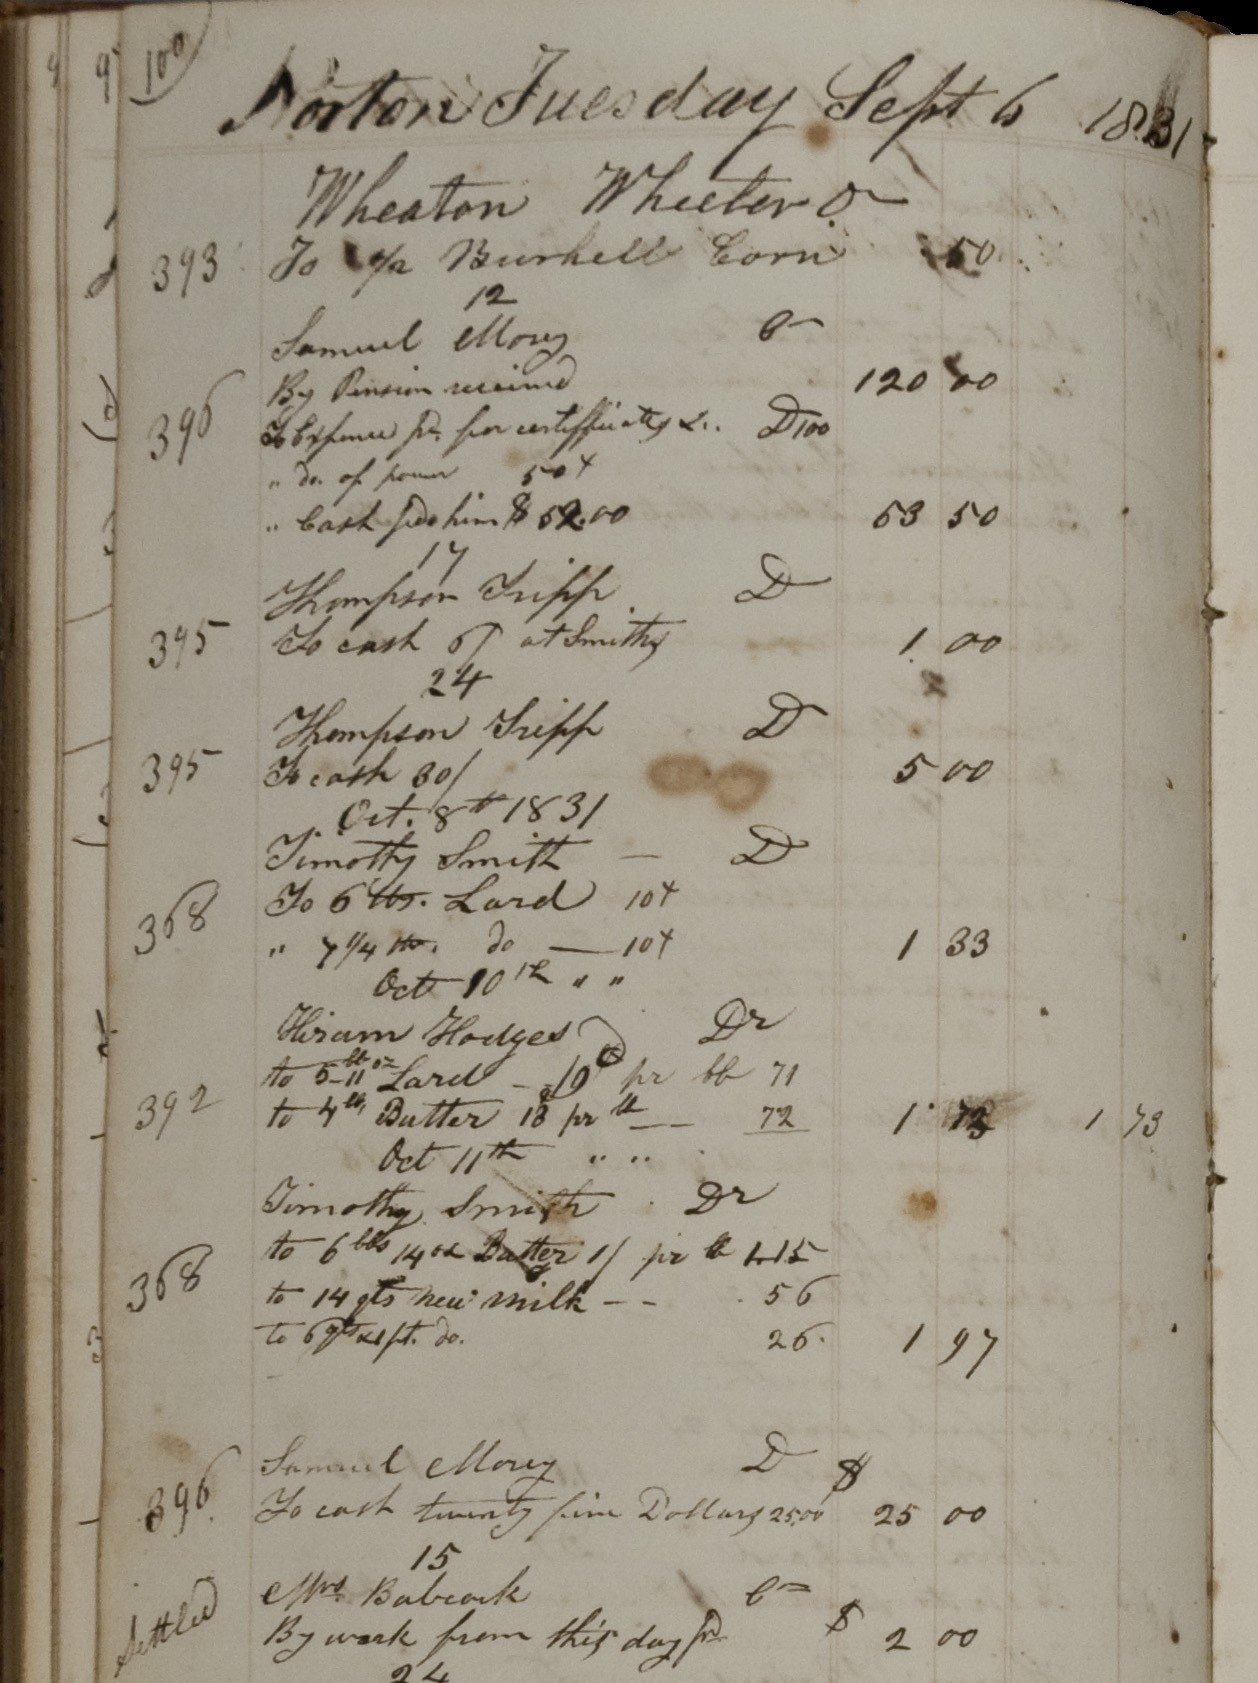
\includegraphics[width=1\textwidth]{img/wheaton_100_101.jpg}  
    \caption[Seite 100 des \textit{Daybook, \protect\url{http://hdl.handle.net/11040/17982}}, 1828-1859]{Seite 100 des \textit{Daybook}, 1828-1859a} \label{fig:wheaton}
\end{figure}
\\
Die vollständige Transkription der ersten 8 Einträge der Seite 100. Diese zeigen die soeben beschriebenen Strukturen.
\\
\\
\begin{tabular}{clcc}
 \textbf{Norton Tuesday Sept 6 1831}\\
    & Wheaton Wheeler & &\\
393 & Dr To 1/2 Burhell Corn & & 50 \\
    & 12 & &\\
    & Samuel Morey  Cr  & &\\
396 & By pension received & 120 & \\
    & To Expense pd. for certificates L. D100 & &\\
    & "Do. of power 50x & &\\
    & " Cash pd. him \$62.00 & 53 & 50\\
    & Thompson Tripp  DR  & &\\
395 & To cash 6/ at Smiths & 1 & 00\\	
    & 24 & &\\
    & Thompson Tripp  DR & &\\	
395 & To cash 30/ & 5  & 00\\		
Oct. 8th 1831\\
    & Timothy Smith DR & &\\
368 & To 6 lb. Lard 10x 6 lb. Lard"7 1/4 lb do 10x & 1 & 33 \\
Oct 10th " "\\
    & Hiram Hodges Dr & &\\
392 & To 5 lb11 oz Lard - 19d pr lb\\
    & 71 5 lb11 oz Lard To 4 lb Butter 13 pr lb 72 & 1 & 73\\
Oct. 11th " "\\
    & Timothy Smith  Dr& &\\
368 & To 6 lbs 14 oz Butter 1/ pr lb 1.15 & & \\ & To 14 Qts New Milk 56 & &\\
& To 6 Qts \& 1 Pt. do 26 & 1 & 97 	\\	
    & Samuel Morey DR & &\\
396 & To cash twenty five dollares 25.00 & 25 & 00\\
    & 15 & & \\	
    & Mrs. Babcock DR  & & \\		
Settled & By work from this day pd & \$2 & 00
\end{tabular}
\\
\\
TOMASEK verfolgt dabei einen TEI/XML-Ansatz, um drei Ebenen dieser Quelle zu beschreiben. Das Layout, die textuelle Struktur der Quelle und die abstrakte Ebene, inhaltliche Ebene der Transaktionen. Letztere ist nur schwer durch die TEI Markup beschreibbar.
\\
Es erweitert den Bereich der Fragen zu historischen Narrativen und geografischen Informationen. Es ist interessant zu folgen.
eine Person oder eine Familie, wie sie im Laufe der Zeit im Tagesbuch erscheinen und ihre Lebensweise rekonstruieren. 
sozialer Hintergrund für eine historische Erzählung. Gleiches gilt für geografische Informationen.
die Möglichkeit, geografische Beziehungen von Personen oder die Herkunft von Waren zu verfolgen.
\\
\\
Ziel der Masterarbeit soll es nicht sein die Projektinhalte zu dokumentieren, sondern sich mit theoretischen und praktischen Fragestellungen zu formaler Modellen und formaler Methoden in den Geschichtswissenschaften  auseinanderzusetzen, wiewohl Quellen, Workflows und Daten aus dem DEPCHA Projekt einfließen sollen.

\section{Digitale Edition von historischen Rechnungsbücher}
\label{subsec:DigEdHiRe}

hehe\footcite[Vgl.][]{sahle2013digitale}
huhu\footcite[Vgl][S.234-252]{jannidis2017digital} 

\subsection{Digitale Edition}
Kapitel in dem digitale Edition, TEI und How to Bookkeep behandelt wird. Und die besonderheiten editorische Arbeit mit Rechnungsbüchern. 

TOMASEK und BAUMAN beschreiben ein Modell eines interpretativen Markups, um Beziehungen zwischen Individueen, Geld- Güter- und Dienstleistungstransfer, die Doppeleintrag-Buchhaltung umfassenm auszuzeichnen. Die Auszeichnung basiert auf den ausdrucksstarken Richtlinien der TEI. \footcite[Vgl.][S.1-2, \protect\url{http://journals.openedition.org/jtei/895}, 08.03.2018]{tomasek2013encoding}
\footcite[][S.41-44]{kobler2010qualitat}

\section{Ein Informationsmodell, formales Modell, konezptuelles Modell  für Rechnugsbücher: die Bookkeeping Ontology}

Im Zuge des Projektes \textbf{Digital Edition Publishing Cooperative for Historical Accounts (DEPCHA)}\footnote{\url{gams.uni-graz.at/depcha}} wird ein gemeinsamer Publikations-Hub für historische Rechnungsbücher umgesetzt. Im Zentrum steht die Entwicklung und Nutzung einer Ontologie zur Formalisierung und Standardisierung von Buchungstransaktionen in historischen Rechnungsunterlagen, sowie ein \textit{Linked Open Data} Zugang. Der Mehrwert entsteht durch Funktionalitäten des Retrievals, der Visualisierung und Analyse der eingespielten Datenbestände.
\\
Für alle diese Projekte existieren hochstrukturierte RDF-Daten, die jeweils mit einer domänenspezifischen Ontologie beschrieben sind. Diese Ontologie wurde in einem iterativen \textit{Ontology Enginneering}-Prozess mit den FachkollegInnen, basierend auf den fachspezifischen Forschungsfragen, generiert.
\\
Das \textit{Data for History Consortium}\footcite{beretta2017dataforhistory} geht einen vergleichbaren Weg und versucht ein gemeinsames Set an Methoden im \textit{Web of Data} zu entwickeln, um Daten in den Geschichtswissenschaften zu modellieren, verknüpfen und auszutauschen.
\\
The common knowledge domain of these documents is formalized in a ”bookkeeping” ontology, based on the REA model and compliant with the CIDOC CRM. As a conceptual data model, the ontology is developed in an iterative process. It formalizes the interpretation of transactions of money, commodities and services from one actor to another, and further properties that can be found in historical accounts. The RDF data extracted from the accounts becomes therefore a highly structured and self describing data set, being interoperable and reusable for researchers in diverse fields. The RDF representation can link to URI’s of commodities, places, persons or other LOD vocabularies. Additionally the RDF representation contributes to the LOD. Thus, all formal methods applied in the DEPCHA project can be transferred to other data conforming to the proposed ontology and any kind of combined data set.

\section{Linked Open Data und Geschichte}

\section{Zusammenfassung}

\newpage
\bibliographystyle{jurabib}
\bibliography{literatur}
\newpage
\listoffigures

\end{document}
